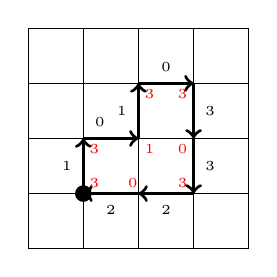
\begin{tikzpicture}[scale=0.7]
	% Grid
	\foreach \x in {0,1,2,3,4} {
	\draw (\x,0) -- (\x,4);
	\draw (0,\x) -- (4,\x);}
	
	% starting point and arrows
	\node[circle,fill=black,inner sep=0pt,minimum size=6pt] at (1,1) {};
	\draw[very thick,->] (1,1) -- (1,2);
	\draw[very thick,->] (1,2) -- (2,2);
	\draw[very thick,->] (2,2) -- (2,3);
	\draw[very thick,->] (2,3) -- (3,3);
	\draw[very thick,->] (3,3) -- (3,2);
	\draw[very thick,->] (3,2) -- (3,1);
	\draw[very thick,->] (3,1) -- (2,1);
	\draw[very thick,->] (2,1) -- (1,1);
	
	% chain codes
	\node at (0.7,1.5) {\tiny 1};
	\node at (1.3,2.3) {\tiny 0};
	\node at (1.7,2.5) {\tiny 1};
	\node at (2.5,3.3) {\tiny 0};
	\node at (3.3,2.5) {\tiny 3};
	\node at (3.3,1.5) {\tiny 3};
	\node at (2.5,0.7) {\tiny 2};
	\node at (1.5,0.7) {\tiny 2};
	
	% first order difference
	\node[color=red] at (1.2,1.2) {\tiny 3};
	\node[color=red] at (1.2,1.8) {\tiny 3};
	\node[color=red] at (2.2,1.8) {\tiny 1};
	\node[color=red] at (2.2,2.8) {\tiny 3};
	\node[color=red] at (2.8,2.8) {\tiny 3};
	\node[color=red] at (2.8,1.8) {\tiny 0};
	\node[color=red] at (2.8,1.2) {\tiny 3};
	\node[color=red] at (1.9,1.2) {\tiny 0};
	
\end{tikzpicture}